\documentclass[minf,frontabs,twoside,singlespacing,parskip]{infthesis} % 

%\usepackage{biblatex}
\usepackage[xetex]{graphicx}
\usepackage{url}
\usepackage{fontspec,xunicode}

\defaultfontfeatures{Mapping=tex-text,Scale=MatchLowercase}
\setmainfont[Scale=.95]{Georgia}
\setmonofont{Georgia}

\usepackage{amsmath}
\newcommand{\BigO}[1]{\ensuremath{\operatorname{O}\bigl(#1\bigr)}}

\begin{document}
\title{Modelling search volumes as a dynamic system responding to external events}

\author{Stefan Sabev}

\course{Master of Informatics}
\project{{\bf MInf Project (Part 1) Report}}

\date{\today}

\abstract{
It is well known that some events might spark people's interest to fly to different destinations. In particular news events or sports events can quite easily make people search for a specific destination - for example the Champions League Quarter final draw increased the number of flight searches from Glasgow to Spain 6 times.\\
For this project we have collected vast amounts of Twitter data. With this dataset and the flight search dataset provided by Skyscanner it was possible to build a classifier that predicts flight search demand based on what's happening on Twitter. This is a noble approach to predicting flight search volumes utilising the vastness of Social data available. \\
The potential applications of this are generic prediction of flight search volumes, predicting new events for better marketing and also anomaly detection in traffic caused by events.
%The main goal of this project is to collect Twitter data initially and possibly several other news sources and extract the available event data. Afterwards we'd want to split it into two groups - those who spark people's interest and those don't.
%This can later be used to detect when people want to go somewhere based on the news channels around the world.
}

\maketitle

\section*{Acknowledgements}

I would like to thank Charles Sutton for his support while supervising this project.\\
\\
Another thank you to Ewan Nicolson for helping with the project and giving access to data storage and the Skyscanner dataset used in this project.

\tableofcontents

\pagenumbering{arabic}

\chapter{Introduction}

With millions and some with even billions of users, Social Networks are becoming an increasingly more important in our lives. A big proportion of people use it as their primary way of communicating with the outside world. As with any other network - be it TV, radio, newspaper - people are trying to benefit in some way from it. Due to the vastness of its data, this new generation of networks has created an entirely new ecosystem of its own - companies are doing sentiment analysis, targeted ads, clustering and segmentation of customers being prime examples of this. 

One of those social networks is Twitter {\copyright}. With a base of 200 million active users it has slowly become a very promising source of data after they opened up their public streams. There are lots of articles which are using it to do plenty of amazing things - demographics research, predicting flu outbreaks, etc. \cite{TwitterResearch}

The aim of this project is to explore what is the effect that social media and more specifically Twitter has on online travel. We are trying to show that using Twitter we can build a model that will be able to predict some certain upward and possibly downward shifts in demand on airline routes. 

In order to get more familiar with the trending events I have done read a few papers on Topic Detection and Tracking and First News Detection in order to see if I could use and extend it for my case. I'd like to mention Sasa Petrovic's PhD thesis as an excellent paper on the matter\cite{Petrovic2012}.

There aren't that many flight search companies out there and up to this day there hasn't been any research into this particular topic. That is quite possibly due to the fact that it is a ver niche are and mod of the flight search datasets are not publicly available. The lack of data and the closed nature of the Online Travel industry have made research like this impossible until now. 

Skyscanner has always been a data-driven company. It's one of the few companies in this industry that is still growing at a massive rate. That growth is the same as far as their data is concerned - the company is serving billions of searches every month. 

\chapter{Methodology}

%The problem we have at hand is completely new. 

Since the problem we face here is completely new, I had to delve into the data and explore the data as much as possible in order to understand the data set and find out what we can use in order to do our predictive modelling.

I have tried several different approaches to filtering the data and exploring the relationship between the two variables. The ones worth mentioning are:
\begin{itemize}
\item Using hashtags which contain a country or city name and taking their counts.
\item Taking every tweet that has a city/country name in its text in a conduction with a travel related term from the list. 
\end{itemize}

Another important aspect of the project is to take care of the data. Because of some teething problems both with the Skyscanner data and the Twitter Streaming API, there are some holes in it, which I have chosen to remote by filling in data generated by the Last 4 Fridays forecasting method. 


\section{Data collection}

The first and most important part of this project was to start collecting the correct data, which was to be used in building the model later. Twitter offers quite a comprehensive API with a lot of attributes, however in order to reduce the daily volume of data I had to take the most relevant ones for me. 

The attributes chosen to collect are:
\begin{itemize}
\item Text - the text of the tweet is the most important one, perhaps. Quite a lot of information can be extracted from it alone
\item Id - the tweet id. Useful if we want to screen scrape for any additional information or just to provide a tidy small dataset of ids.
\item ID Str - String representation of the above.
\item Source - What is used to post the tweet. The Twitter website is marked as "web".
\item Coordinates  - Representation of the geographical location of the Tweet as reported by the utility used to post the tweet.
\item Entities - This include hashtags, user mentions and urls included in the tweet. Could be taken from the text, but it's nicer to have them ready.
\item Retweet count - the number of times the tweet was retweeted. Useful for any future models. 
\item Favourited - Indicates whether the tweet was favourited by people - an analogy of this would be a Facebook like. 
\item Language - The language of the tweet. We are capturing English language tweets at the moment, but put in place for future expansion into the multi-language domain
\item Filter level - indicates the level of filtering applied to the stream.
\item Place - Shows where the tweet was tweeted from. Gives more detail than coordinates - country, city name, coordinates as well. Not necessarily available for all tweets.
\end{itemize}

The first stage of the project is to look only at tweets in English coming from the UK. That will allows us to predict and model the flight search volumes in the UK based on the mentions in the Twitter Stream.

The second stage would be to develop the model even further and add multi-language and multi-country support and employ more sophisticated models such as ARIMA or Auto-regressive Vector Models.

By selecting those particular tweet attributes and using the Streaming API, I managed to reduce the daily volume of data from \textasciitilde 6GB of data down to \textasciitilde 3.5GB/day.
The amount of data accumulated at the time of writing is \textasciitilde 380 GB. The collector has been running successfully from September 2013, however there are some holes of the data caused by network outages or the script interacting with the Twitter Streaming API crashing. 

The data on flight search volumes is kindly provided by Skyscanner. In order to ensure that there are no concerns with confidentiality I have anonymised the data. 

\section{Hashtags}

Hashtag is one of the most important constructs by Twitter. Here's an example tweet:

\begin{quotation}
@FunnyChap: Something witty and very well said \bf{\#jokeoftheweek}
\end{quotation}

The structure of the tweets is:
\begin{enumerate}
\item The name of the user is denoted with a @ before the username.
\item The text itself.
\item The hashtag (a special Twitter construct) is denoted with a \#.
\end{enumerate}

You can filter out and explore twitter content based on hashtags and usually every major event has its own hashtag. The ones which are most mentioned appear in a special section called "Trending".

This option was considered, because if it had worked it would have been what we would call a "quick win". It doesn't require much processing, since what you'd need is just take the ready made list of hashtags and store all the results into a in-memory dictionary, which you'd then split by city/country. That reduced the overall size of the relevant tweets to \textasciitilde 3 GB. What was even greater is that we didn't really require the text information itself, which made the working dataset even smaller. 

However the overall counts were quite small and the distribution of the values was very noisy, which means that fitting a model to this would've been quite hard if not impossible.

\section{Occurrences paired with travel terms} 

The next slightly more expensive in computational terms option was to look at the actual tweet content and to count the number of times a city/country name appeared in conjunction with a one word form a list of travel-related words:

\begin{quotation}
terms = \\
\{ "airport": "", \\
"check-in": "", \\
"fly": "", \\
"land": "", \\ 
"landing": "", \\
"plane": "", \\ 
"take off": "", \\
"destination": "" \\
... \}
\end{quotation}

The list is modelled as a dictionary, because dictionary lookups are \BigO{1}, so iterating over the words in the tweet and checking whether they appear in the city/country dictionary or the travel terms proved to be the most efficient combination.

That gives us about  \textasciitilde  10 GB of tweets to work with. The reduced dataset is still much smaller in comparison to the full one. Processing the whole usually takes about a day, because of the extensive lookups in the city/country dictionary and the travel terms one.

\section{Finding the correlation between those variables}

After discovering that the volumes of twitter counts from the second method are not so noisy, I decided to proceed and explore the correlation between the two variables.

The easiest way to test the statistical correlation between your data would be to carry out the Pearson test.

For London the numbers we got back from that are:
\begin{quotation}
In [39]: r\_row, p\_value

Out [39]: (0.13, 0.28)
\end{quotation}

From this it seems that the situation is truly unrelated. After all a positive correlation of only 13\% is something that even a social scientist wouldn't report!

However, when you plot the two things we are trying to correlate something a bit more interesting comes up:

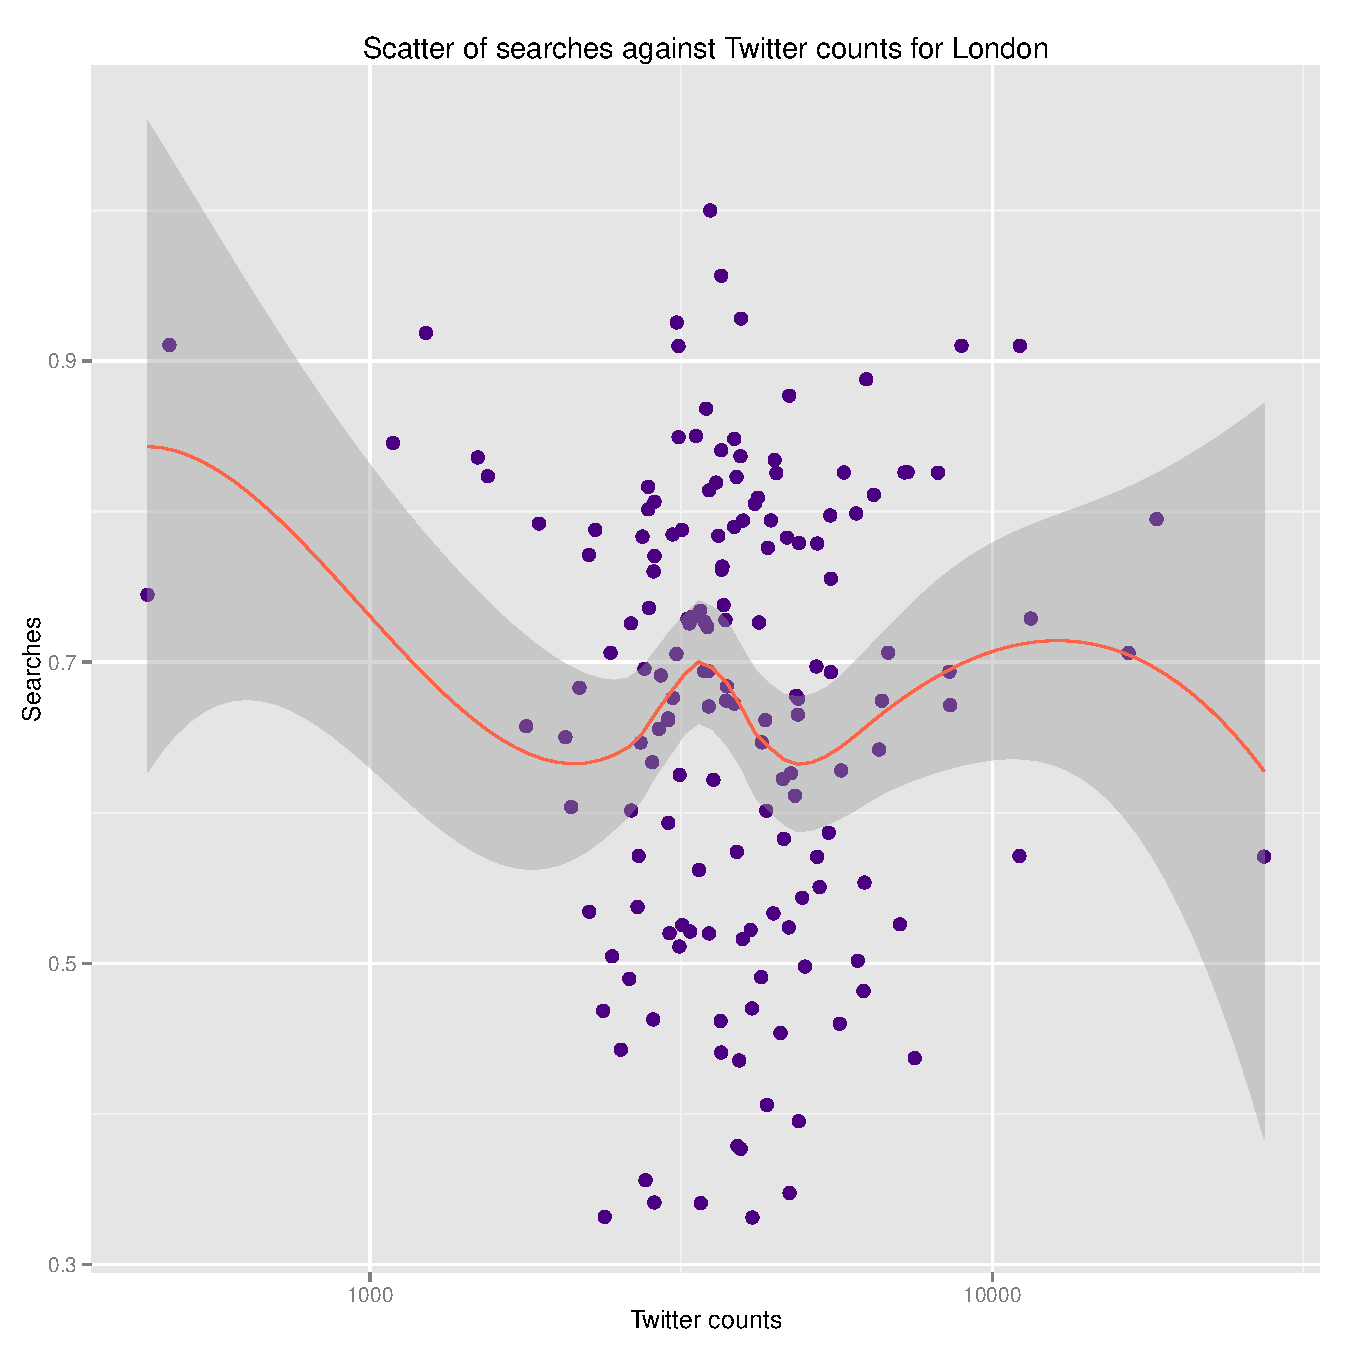
\includegraphics[width=\textwidth]{London}

There is definitely a relationship, even though not perfectly linear.

We can observe that there is a well defined cluster where the twitter counts are big and the corresponding searches are relatively big as well. We can't say with great certainty that those two are perfectly correlated, because correlation does not imply causation. So what we needed to do was to delve even further and build a model that would work with those.

%So we can certainly say that those variables are correlated, but the outliers push the coefficient down quite a significant amount. The interesting part of this scatter plot for us is the top right corner. We are interested in those abnormal Twitter counts, which correspond to high number of redirects. Another interesting thing to explore would be to see if we correlate the mentions on the social network with the redirects from the next day. That will assume a certain lag factor, which is reasonable as sometimes an event should not effect the redirect counts till the next day when it's picked by all the major media. 

Paris was one of the most popular destinations so it was quite interesting to see what the relation is there. The Pearson test yields the following values for Paris:
\begin{quotation}
In [24]: r\_value, p\_value

Out[24]: (-0.25, 0.0047)
\end{quotation}
\newpage
And here is the scatter plot:

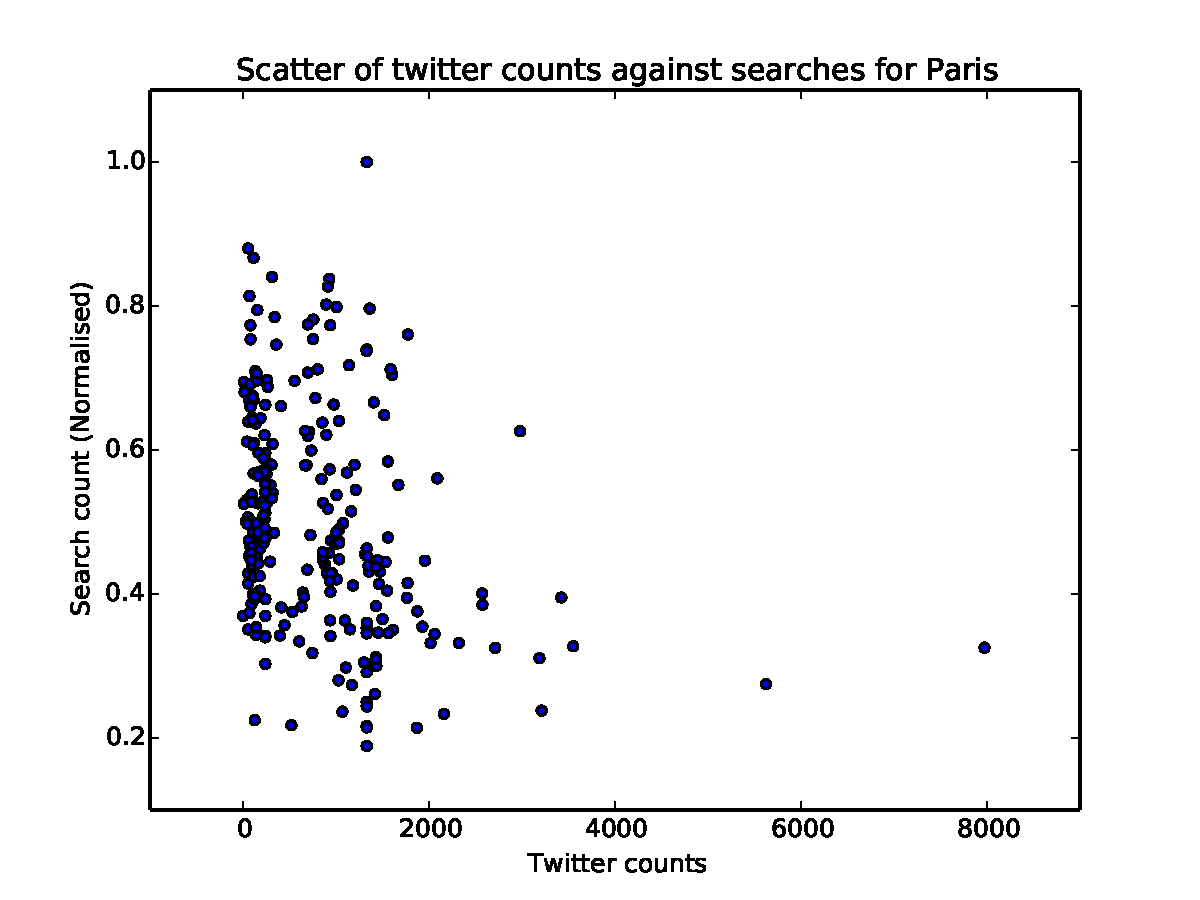
\includegraphics[width=\textwidth]{Paris}

Here we do see that indeed the correlation is relatively small and negative. 

As we can see each of the different cities shows a different behaviour. The implications of that are that the approach we take to building the model must be more versatile - we will aim to build one model for the overall numbers and models on a per city basis.

\section{Cleansing the data}

As mentioned, every time you depend a few external data source there will be some problems with the data, caused by several things. 

In this project there were a couple of major sources of problems:
\begin{enumerate}
\item The script that collects data from the Streaming API.
\item The searches data coming from Skyscanner being incorrect or partial - not spanning the full date range.
\end{enumerate}

The dates with incomplete data or missing data altogether can seriously impact any regression or statistical test, so it was vital to tidy up the data set by backfilling it. I applied the Last 4 Fridays forecasting algorithm mentioned in the following chapter in order to make the dataset more consistent and easier to work with. 

The interesting part was that it completely change the results from the test. For London the values returned by the Pearson test are now:

\begin{quotation}
In [23]: r\_row, p\_value

Out[23]: (-0.23, 0.02)
\end{quotation}

That is quite interesting and it has a lot of implications on the models we will use afterwards to correlate the two variables. 
We might have to add a certain "lag" factor to this, which will offset the tweets by correlating the numbers extrapolated from Twitter with the numbers and match them against searches from the following day.

%\section{Top features} 

%The idea here is to extract the top N features from the tweet and use them in the logistic regression model that we will build to predict the search counts. I plan on working on this in the next couple of weeks.


\chapter{Models}

\section{The baseline model}

The baseline model for predicting the number of redirects Skyscanner has on a daily basis is called Last 4 Fridays. 
It works in the following way:
\begin{enumerate}
\item We want to predict the number of redirects/searches for this Friday.
\item We take the number of redirects/searches Friday from last week, the week before, etc, until we have the counts form the previous 4 weeks for the corresponding day.
\item We then assign weights to those 4 numbers and assign weights - the most recent one will get the highest weight, the one after about a half and so on. The exponential weighting scheme captures short term seasonality.
\end{enumerate}

This model was tested out against more complex classifiers like ARIMA and Autoregressive Vector Methods and it performed really well, but unlike the others it was many times simpler to program and maintain.

\section{Last 4 Fridays + Twitter Counts}

The first model I build was not a radical new approach, but rather an increment on the previous one.

I generated a list of tuples which contained the following information:
\begin{itemize}
\item Twitter count for the place - how many times it was mentioned in conjunction with a travel term.
\item Same day of the week from last week
\item Same day of the week from 2 weeks ago
\item Same day of the week from 3 weeks ago
\item Same day of the week from 4 weeks ago
\end{itemize}

What this is is a version of Last 4 Fridays which now has Twitter Counts. Instead of using the exponential weights from the previous algorithm I let LASSO determine their weights.
With LASSO I had weights for each of the 272 cities. After measuring the RMSEs for the L4F algorithm and expanded version with Twitter Counts the former performs better on 193 of the 272 cities. In the top 10 L4F+Twitter performs better on 2 out of 10. 

Dublin which is in the 4th spot in terms of volumes is quite interesting. I plotted out the counts against searches just to see how it looks:

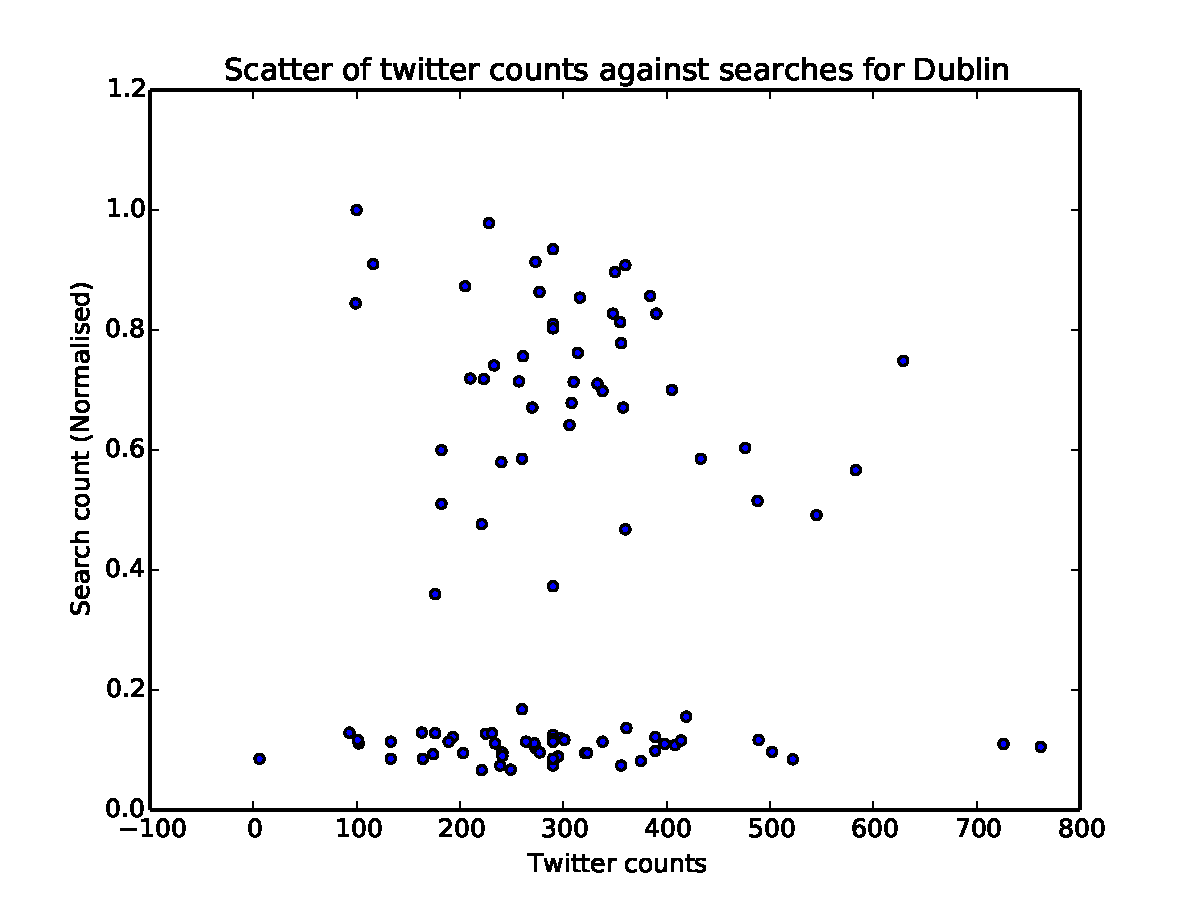
\includegraphics[width=\textwidth]{Dublin}  

\newpage
\section{Results}

And here are the results for the top 10 destinations by volume (they have the highest RMSEs).

\begin{tabular}{ l | r | r }
City	& RMSE L4F+Twitter &RMSE L4F \\
\hline
London & 3335.869525 & 3160.05886 \\
Paris	 & 939.1057276 & 921.6785638  \\
Barcelona & 920.6831066 & 897.6473097  \\
Milan & 760.3436591 & 760.9286718  \\
Rome & 710.7052517 & 705.8388511  \\
Manchester & 574.8431422 & 572.4116201  \\
Dublin & 514.584231	 & 527.884409  \\
Amsterdam & 550.2254781 & 516.2054596  \\
Tenerife & 544.6187529 & 502.0270723  \\
Moscow & 499.1803266 & 495.2139406  \\
\end{tabular}


This is quite a good start considering the fact that all the weights were automatically determined by the LASSO algorithm and the fact that I have only about 130 data points so far (130 days).

\section{Future improvements}

The next on the list is to expand the feature set with more features from Twitter such as:


\begin{itemize}
\item Specific words.
\item Trending event or not.
\item Investigate whether sentiment will be useful here.
\end{itemize}

With those I'll be able to better the model and reduce the RMSE across the whole board and hopefully beat the current prediction algorithm for more than 80\% of the examples.


\chapter{Timeline}

The timeline for the next 3 months is the following:
\begin{enumerate}
\item Better the existing model and continue with the tests. .
\item Add more features to the set of inputs.
\item Work on both approaches:
\begin{itemize}
\item Explain spikes in searches by looking at historical tweet data
\item Or try to predict the spikes in the first place
\end{itemize}
\item Final draft done by mid-March.
\item Submit dissertation the final week of March.
\end{enumerate}

\bibliographystyle{ieeetr}
\bibliography{Master}

\end{document}
